\chapter{Étude hydrodynamique}
\section{Expérience numérique}

L'objectif est de réaliser numériquement l'expérience proposée par Abhijit Rao et al. dans \cite{rao_influence_2015}. Pour cette expérience une goutte composée d'Acetonitrile et de Chlorobenzene est placée dans de l'eau. l'acetonitrile est miscible dans l'eau contrairement au chlorobenzene qui est immiscible. Initialement la goutte est plus légère que l'eau environnante et monte puis sous l'effet du transfert de masse la densité de la goutte augmente jusqu’à une inversion du rapport de densité conduisant à la redescente de la goutte.
\subsection{Choix des conditions initiales}
Les conditions initiales choisies pour la concentration sont de la forme tangente hyperbolique.
\begin{equation}
	\phi_{i}(\mathbf{x},t=0) = \frac{\phi^{init,cont}_i + \phi^{init,disp}_i  }{2} +  \frac{\phi^{init,cont}_i - \phi^{init,disp}_i }{2}\tanh\left(\cfrac{\sqrt{(x-x_0)^2+(y-y_0)^2}-R}{\varepsilon} \right)
\end{equation}
Avec ($x_0$, $y_0$) les coordonnées du centre de la goutte, $R$ le rayon de la goutte, $\varepsilon$ l'épaisseur de l'interface (paramètre numérique) et $\phi_i^{init,cont}$ (resp. $\phi_i^{init,disp}$) la concentration initiale de l'élément $i$ dans la phase continue (resp. dispersée) .\\
Cette solution analytique provient d'un problème avec une interface plane (sans courbure), dans la littérature il n'existe pas de solution analytique pour une interface courbée, l'effet de Gibbs-Thomsom n'est donc pas pris en compte, ainsi on observe un léger mouvement de l'interface lors du premier pas de temps. \\
Pour s'assurer de la sphéricité de la goutte lors de la simulation on calcule le nombre adimensionné de Bond  représentant le ratio entre les forces de gravité et la tension de surface tel que :
\begin{equation}
	Bo = \cfrac{\Delta \rho g D^2}{\sigma}
\end{equation}
avec $\Delta\rho$ la différence de densité entre les deux phases, $D$ le diamètre de la goutte et $\sigma$ la tension de surface.\\
On considère que pour $Bo \ll 1$ la tension de surface domine et la goutte reste sphérique.
\begin{figure}[H]
	\centering
	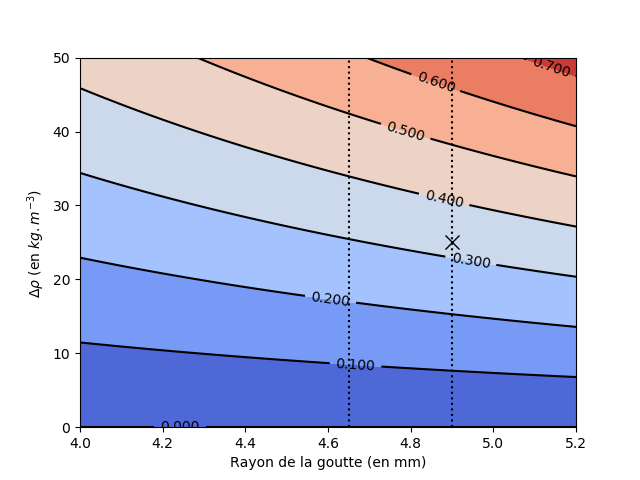
\includegraphics[width=0.7\linewidth]{figure/contour_bond}
	\caption[Valeur du nombre de Bond en fonction de la différence de densité et de la tension de surface entre les phases]{Valeur du nombre de Bond en fonction de la différence de densité entre les phases et le rayon de la goutte, le marqueur représente l'état initial}
	\label{fig:contourbond}
\end{figure}
Il est alors possible, dans notre cas, de discuter de la sphéricité de la goutte au vu de la valeur ici $Bo = 0.32$
